\setlength{\parskip}{0.5em}
\section*{Einleitung}
    Zu einem modernen Automobil ind heute Assistenzsysteme selbstverständlich. Immer mehr werden dabei auch Assistenten eingesetzt, welche anhand von Kamerabilder, den Fahrer ünterstützen.
    Neben Rückfahrkameras, Spurhalte- oder Nachtsicht-Assistenten, werden auch vermehrt Assistenten eingesetzt, welche Verkehrszeichen Detektieren und Klassifizieren.

    Eine automatische Verkehrszeichen-Erkennung, kann Fahrern dabei helfen tempolimits einzuhalten, oder verpasste Verkehrszeichen nachzuschauen und kann somit helfen richtige Entscheidungen
    während des Fahrens zu treffen.

    Im Rahmen eines Praktikums an der Eberhard Karls Universität Tübingen, soll eine automatische Verkehrszeichen-Erkennung für Mobiltelefone entwickelt werden. Dabei sollen insbesondere
    Methoden der Bildverarbeitung und des Maschinellen lernens eingesetzt werden. Das Praktikum wird von Prof. Schilling und seinem Team, am Lehrstuhl Graphisch Interaktive Systeme am 
    Wilhelm Schickard Institut für Informatik, betreut.
\section*{Praktikumsprojekt}
    Im folgenden wird das Projekt kurz beschrieben. Neben den Zielen werden erste Konzepte sowie ein Arbeitsplan vorgestellt.
\subsection*{Produkt}
    Ziel des Projekt ist es einen kamerabasierten Fahrassistenten zu entwickeln, welcher sich auf einem Smartphone befindet. Der Fahrassisten soll die Kamera des Smartphones benutzen,
    um in Fahrtrichtunge Verkehrszeichen zu erkennen. Erkannte Verkehrszeichen sollen dem Fahrer für eine gewisse Zeit angezeigt werden und ihm somit helfen, möglichst wenig Verkehrszeichen zu
    verpassen.

    Smartphones welche GPS bereitstellen, sollen zusätzlich eine Warnung ausgeben, falls ein erkanntes Tempolimit überschritten wird.
\subsection*{Umsetzung}
    Als Smartphone Plattform wird Android eingesetzt. Entsprechend wird die Applikation im wesentlichen in Java entwickelt werden. Android stellt bereits eine Java-Schnittstelle zur Grafik-Library
    OpenCV. Je nach eingesetztem Smartphone ist es dadurch möglich, einfach und schnell, Bildverarbeitung auf der GPU auszuführen.

\subsubsection*{Pipeline}
    \begin{itemize}
        \item Auslesen des Kamerabildes vom Smartphone.
        \item Extrahieren der relevanten Bildbereiche (Schilder befinden sich i. d. R. rechts der Fahrtrichtung, oder beidseitig).
        \item Erkennen von Schildern.
        \item Erkannte Schilder klassifizieren.
        \item Klassifiziertes Schild anzeigen.
        \item Ggf. Fahrer akustisch und/oder visuell über Geschwindigkeitsübertretung warnen.
    \end{itemize}
    \begin{figure}
            \centering
            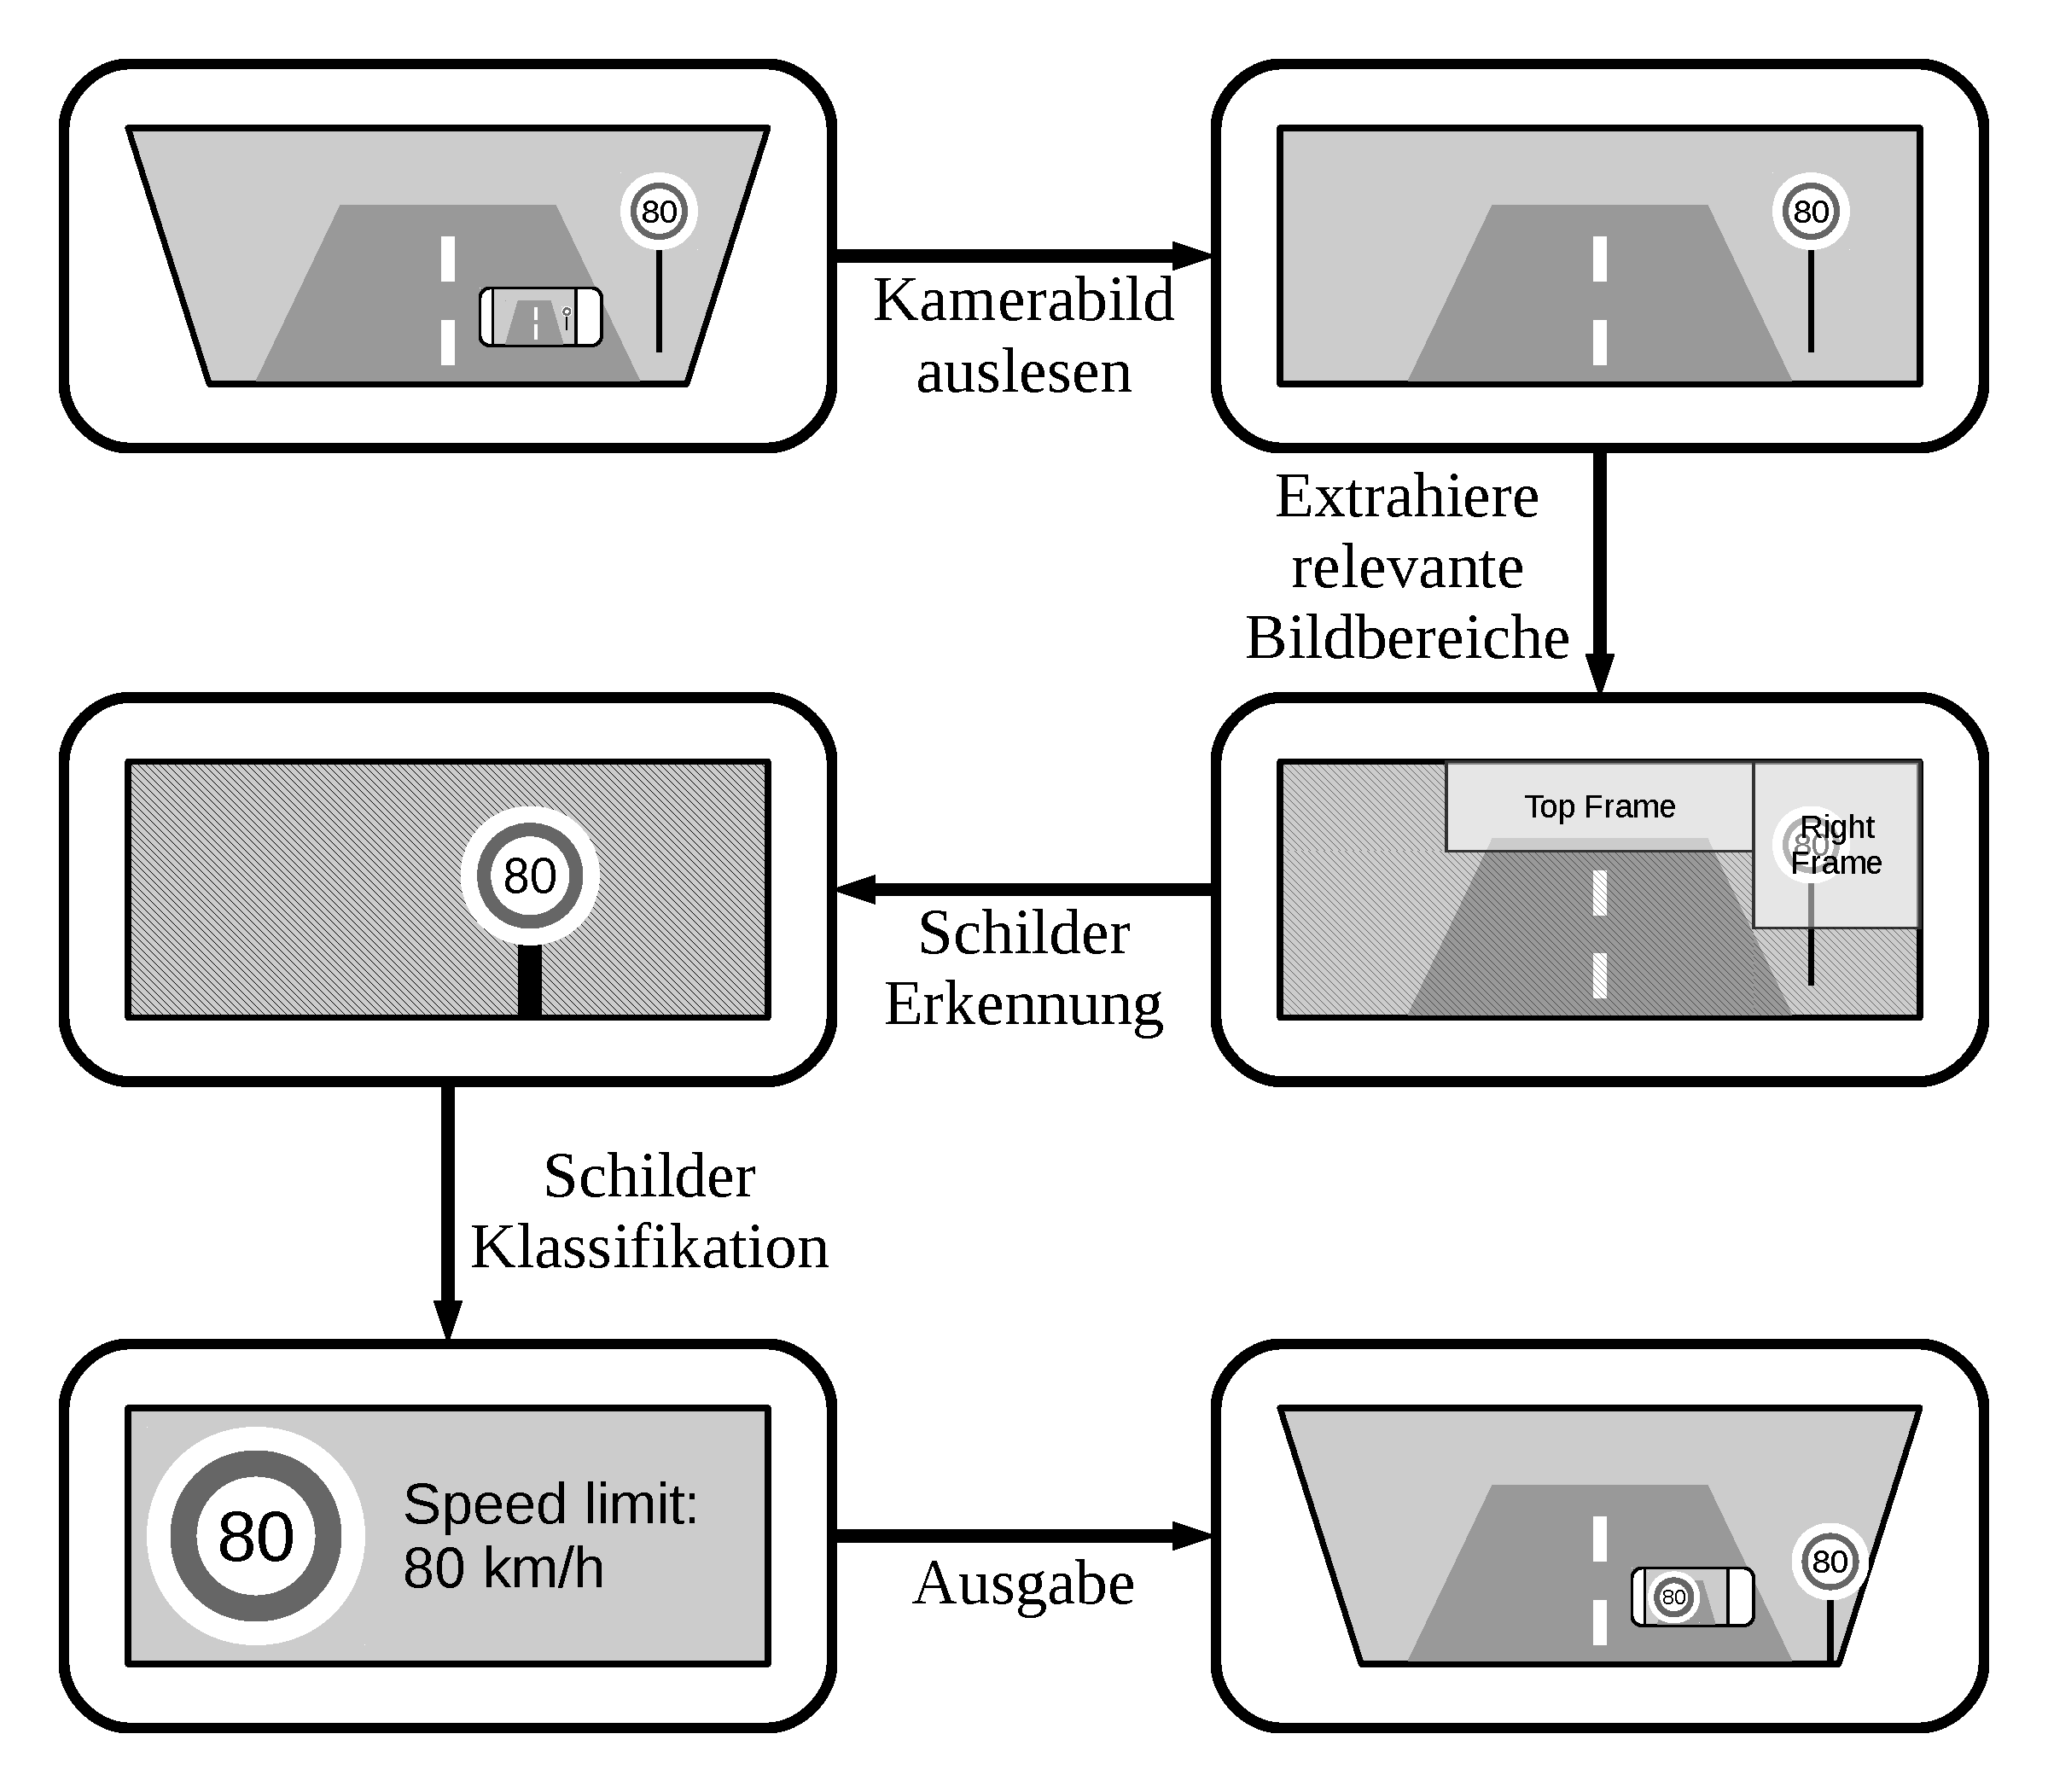
\includegraphics[width=0.75\textwidth]{pipeline.pdf}
            \caption{Pipeline}
    \end{figure}
\subsection*{Algorithmen}
    Der Kern der Anwendung kann in zwei grundlegeden Schritte eingeteilt werden:
    \begin{description}
        \item[Schilderkennung (Traffic Sign Detection):]
            Die Aufgabe der \emph{Traffic Sign Detection} ist es in einem Bild Schilder zu erkennen.
            Die relevanten Bildausschnitte werden extrahiert und an den \emph{Traffic Sign Recognition}
            Algorithmus übergeben.

            Da dies in Echtzeit auf einem Smartphone geschehen soll, müssen die verwendetetn Verfahren
            möglichst schnell sein.
            
            Erste versuche, über Farbkanal und Hough-Transformation Runde (Elliptische) Schilder zu 
            erkennen funktionierten für Schönwetter-Landschafts-Fahrten gut.
            Scheiterten aber falls das Bild eingetrübt ist (z.B. durch Regen, Dämmerung).

        \item[Schilder-Klassifizierung (Traffic Sign Recognition):]
            Die Klassifizierung der Schilder geschieht über Neuronale Netze.
            Auf \url{http://benchmark.ini.rub.de} werden Trainingsdaten bereitgestellt.
    \end{description}
\subsection*{Meilensteine}
    Die folgenden Punkte stellen wichtige Schritte zur Abwicklung des Projekts dar. In Klammer
    steht dahinter der dafür zuständige Entwickler.
	\begin{itemize}
        \item Prototypen Entwicklung:
        \begin{description}
            \item[Traffic Sign Detection:] Implementierung der Algorithmen in Matlab. \hfill (Luis)
            \item[Traffic Sign Recognition:] Implementierung der Algorithmen in Matlab. \hfill (David)
        \end{description}
        \item Validierung der Prototypen:
        \begin{description}
            \item[Traffic Sign Detection:] Funktionstest und Tuning. \hfill (Luis)
            \item[Traffic Sign Recognition:] Training und Funktionstest. \hfill (David)
        \end{description}
        Für das Training und den Funktionstest kann das Datenset von \url{http://benchmark.ini.rub.de} verwendet werden
	    \item Implementierung:
        \begin{description}
            \item[Traffic Sign Detection:] Implementierung in Java (evtl. Abhängigkeit zur OpenCV API). \hfill (Luis)
            \item[Traffic Sign Recognition:] Implementierung in Java. \hfill (David)
        \end{description}
        \item User-Interface und Frame-Grabber für Android. \hfill (Luis+David)
	\end{itemize}
